\documentclass[noamsthm,handout]{beamer}
% ,handout,notes=onlyslideswithnotes

\usepackage[center]{tiddemath}
\usepackage{tiddetext}
\usepackage{tiddedae}
\usepackage{parskip}

\usepackage[utf-8]{inputenc}
\usepackage[T1]{fontenc}
\usepackage{textcomp}
\usepackage{wasysym}

%\usepackage{beamerthemesplit}
\usetheme{JuanLesPins}

\usepackage{verbatim}

\title{Shapes}
\subtitle{--- ett hyfsat funktionellt ritspråk}
\author{Henrik Tidefelt}
\institute{LiTH}
\date{\today}

\newcommand{\inEnglish}[1]{(eng: \emph{#1})}

\newcommand{\maincoveringmode}{invisible}
\usepackage[swedish]{babel}

\providecommand{\paragraph}[1]{\textbf{#1}\,}

\newcounter{tmppauses}

\begin{document}

% svenska är förvalt, men det här visar hur man skulle gjort för att byta till det andra språket:
\selectlanguage{swedish}

\frame{%
\note[item]{Hälsa alla välkomna!}%
\note[item]{Presentera mig.}
\note[item]{Mycket hellre frågor under tiden än efteråt.}
\titlepage}

\section*{Översikt}
\frame{\frametitle{Mål}
  Med den här UppLYSningen hoppas jag (kanske lite naivt)
  \pause
  \begin{itemize}[<+->]
  \item Att ni ska få ett hum om vad \Shapes är.
  \item Få höra era invändningar mot designen som den ser ut idag.
  \item Lyckas hitta någon testpilot.
  \item Väcka intresse för utvecklingssamarbete.
  \end{itemize}
  \note[item]{Inget att säga här.}
}

\frame{\frametitle{Plan}
  De stora inslagen idag är:
  \pause
  \begin{itemize}[<+->]
  \item Beskriva hur språkets struktur ser ut idag.
  \item Visa lite av de funktioner som kärnan erbjuder.
  \item Diskutera intressanta utmaningar för framtiden.
  \item Små avstickare med konkreta exempelkörningar.
  \end{itemize}
  \note[item]{Påminn om att man gärna får ställa frågor!}
}

\setbeamercovered{\maincoveringmode}

\section{Introduktion}
\frame{%
  \begin{center}
    {\Huge Introduktion}
  \end{center}
  \note{Då börjar vi\ldots}
}

\frame{\frametitle{Historia}
  \begin{itemize}[<+->]
  \item Hösten 2003: Första kontakt med MetaPost.
  \item Sommaren 2004: Toolbox för plottning i \Matlab tar form.
  \item Hösten 2004: Börjar undersöka möjligheten att ersätta MetaPost.
  \item September 2005: Shapes, då kallat \emph{MetaPDF}, versionshanteras.
  \item Januari 2007: Shapes, då kallat \emph{Drool}, har använts till stort antal figurer i en bok.
  \item April 2007: Kontrollerade tillstånd.
  \item September 2007: Språket heter \emph{Shapes}, och presenteras för första gången.
  \end{itemize}
  \note[item]{Inget att säga här.}
}
\frame{\frametitle{Rötter}
  \Shapes har sina rötter i många av de språk jag varit i kontakt med:
  \begin{itemize}[<+->]
  \item MetaPost
    \note[item]{(en omarbetning av Knuths MetaFont) --- \Shapes kom till när jag ledsnade på MetaPost.}
  \item Scheme
    \note[item]{--- syntax och funktions-begreppet.}
  \item Haskell
    \note[item]{--- för sina rena ideal.}
  \item C++
    \note[item]{--- utmatningssyntaxen.}
  \end{itemize}
  \note[item]{Inget att säga här.}
}
\frame{\frametitle{Alternativ}
  Några andra ritspråk som finns och/eller används idag:
  \begin{itemize}[<+->]
  \item MetaPost
  \item Asymptote
  \item PGF och TikZ
  \item Haskell~PDF
  \item Functional MetaPost
  \end{itemize}
  \note[item]{Inget att säga här.}
}
\frame{\frametitle{Varför \Shapes?}
  Givet utbudet av alternativa rit-språk, varför utveckla ett till?  Här är några skäl:
  \begin{itemize}[<+->]
  \item Inte funktionellt orienterade (alla utom Haskell~PDF och Functional MetaPost).
  \item Dålig beräkningskapacitet (MetaPost och PDF/TikZ).
  \item Saknar domän-specifik syntax (Haskell~PDF).
  \item Inte publicerade när \Shapes påbörjades (Asymptote och Haskell~PDF).
  \item Osmidig arbetsgång (Functional MetaPost).
  \end{itemize}
  \note[item]{Inget att säga här.}
}

\begin{frame}[fragile]
  \frametitle{Hello, shaper!}

\texttt{%
$\bullet$page <{}< [stroke (0cm,0cm)-{}-(1cm,1cm)]
}

% \vspace{5mm}

% \pause

% \texttt{%
% $\bullet$page <{}< stroke [] ((0cm,0cm)-{}-(1cm,1cm))
% }

% \vspace{5mm}

% \pause

% \texttt{%
% [($\backslash$ $\bullet$dst pth .> \{ $\bullet$dst <{}< stroke [] pth \} )\\
% \ \ $\bullet$page \ (0cm,0cm)-{}-(1cm,1cm)]
% }

  \note[item]{Kör live-demo!}
\end{frame}

\section{Språkets struktur}
\frame{%
  \begin{center}
    {\Huge Språkets struktur}
  \end{center}
  \note[item]{Det här är kanske inte den roligaste biten av presentationen för den som är intresserad av grafik.}
}

\subsection{Enkla typer}
\begin{frame}[fragile]\frametitle{Exempel på enkla typer}
  \begin{itemize}
  \item Flyttal: \texttt{14}, \texttt{14.5}, \texttt{~1}
  \item Heltal: \texttt{'5}, \texttt{'$\sim$12}, \texttt{'0xFF}
  \item Längd: \texttt{7cm}, \texttt{$\sim$3mm}, \texttt{72bp}
  \item Sträng (mer detaljer senare): \texttt{\textasciigrave{}Hej!\textasciiacute{}}
  \item Symbol: \texttt{'left}
  \end{itemize}
  \note[item]{Inget att säga här.}
\end{frame}

\subsection{Bindningar och scopes}
\frame{\frametitle{Lexikala bindningar}
  Lexikala bindningar fungerar som i Scheme, men kan inte bindas om.

  \texttt{%
    a{\color{red}:} 42
  }

  \pause
  
  Räckvidden \inEnglish{scope} är begränsad till en kod-klammer \inEnglish{code bracket}:

  \texttt{%
    {\color{red}\{}\\
    \ \ a: 42\\
    \ \ $\bullet$stdout <{}< a\\
    {\color{red}\}}\\
  }

  \note[item]{Inget att säga här.}
}
\frame{\frametitle{Lexikala bindningar --- detaljer}
  
  \begin{itemize}
  \item Högerledet evalueras i samma scope som bindningen tillhör.  (Jämför \texttt{letrec} i Scheme.)\\
    \texttt{%
      odd:  $\backslash$ n .> [if n = '0  false [even n - '1]]\\
      even: $\backslash$ n .> [if n = '0  true  [odd  n - '1]]
    }
  \item Skuggade bindningar kan nås:\\
    \texttt{%
      a: {\color{red}../}a + 7
    }
    \note[item]{Tillgång till skuggade bindningar kräver förståelse av vilka konstruktioner som inför en kod-klammer.}
  \item Se \filename{scopes.drool}!
  \end{itemize}

  \note[item]{Inget att säga här.}
}
\frame{\frametitle{Dynamiska bindningar}
  Dynamisk bindning infördes som ett sätt att undvika den imperativa spagetti-struktur som ett skrivbart \emph{graphics state} lätt kan leda till.

  \texttt{%
    @width:4bp | [stroke mypath]
  }
  
  \begin{itemize}
  \item Dynamiska variabler inleds med \texttt{@}.
  \item Den dynamiska variabeln tillsammans med ett värde blir ett nytt värde som representerar en potentiell dynamisk bindning.
    \note[item]{Förslag på bätte språkbruk?}
  \item Bindningsvärden kan kombineras:\\
    \texttt{%
      @width:4bp \& @dash:[dashpattern 1cm 4mm]
    }
  \item Dynamiska bindningar sätts i scope med en ``pipe''.
  \item En dynamisk variabel har ett filter och ett skönsvärde \inEnglish{default value}.
  \end{itemize}
}
\begin{frame}\frametitle{Dynamiska värden}
  En dynamisk variabel kan bindas till ett \emph{dynamiskt värde}.
  \begin{itemize}
  \item Ser ut så här:\\
    \texttt{%
      @bigmargin: {\color{red}dynamic} 1.3 * @smallmargin
    }
  \item Undviker behovet av att binda alla dynamiska variabler till argumentlösa funktioner.
  \end{itemize}
\end{frame}
\subsection{Funktioner och anrop}
\frame{\frametitle{Funktionsdefinitioner}
  Exempel:

  \texttt{%
    {\color{red}$\backslash$} x y {\color{red}.>} x * x + y * y
  }

  \pause
  \begin{itemize}
  \item Argumentens namn är en del av funktionens signatur.
  \item En slask \inEnglish{sink} kan ta hand om ytterligare argument.\\
    \texttt{%
      $\backslash$ x y {\color{red}<>} rest .> x + y + (foo [] <>rest)
    }
  \item Vilka argument som helst kan få skönsvärden:\\
  \texttt{%
    $\backslash$ x{\color{red}:}3 y z{\color{red}:}2 .> x + y + z
  }
  \end{itemize}
  \note[item]{Inget att säga här.}
}
\begin{frame}\frametitle{Enkla funktionsanrop}
  Ett enkelt funktionsanrop kan ange argument både genom ordning och genom namn.
  
  \texttt{%
    hypot: $\backslash$ x y .> [sqrt x*x + y*y]
  }

  \begin{itemize}
  \item Ordnade argument: se anrop till \texttt{sqrt}.
  \item Namngivna argument: \texttt{[hypot y:3 x:4]}
  \item Blandat: Ordnade argument måste komma först.
  \item Endast ett argument: \texttt{square [] 3} eller \texttt{square [] x:3}
  \end{itemize}
  
  Märk att namngivna argument kan inte ändra betydelsen av ordnade argument!
\end{frame}
\begin{frame}\frametitle{Snitt}
  Scheme: \emph{evaluated cuts}

  \texttt{%
    [hypot 3 ...]
  }
  \\
  \texttt{%
    [hypot y:4 ...]
  }

  \begin{itemize}
  \item Ordnade argument blir helt osynliga i den nya funktionen.
  \item Namngivna argument (er)sätter skönsvärden.
  \item Endast ett argument: \texttt{hypot [...] 3} eller \texttt{hypot [...] y:4}
  \end{itemize}
  
\end{frame}
\subsection{Kontrollerade tillstånd}
\begin{frame}\frametitle{Scenario}
  Utgångsbudet för att skapa en komplex bild i ett funktionellt språk är att skriva ett stort uttryck som sätter ihop de ingående delarna till en helhet.

  \begin{itemize}
  \item Det skapar lätt en krystad struktur i koden.
  \item Det stämmer illa med \emph{painter's model} och hur de flesta av oss tänker på att skapa en bild.
  \item Intuitionen är snarare \emph{imperativ}!
  \item \ldots men variabler kunde ju inte bindas om\ldots
  \end{itemize}

  \note[item]{Inget att säga här.}
\end{frame}
\begin{frame}\frametitle{Kontrollerade tillstånd}
  \Shapes erbjuder \emph{kontrollerade tillstånd} \inEnglish{limited states} för att tillåta en viss grad av imperativ stil.

  \begin{itemize}
  \item Kontrollerade tillstånd binds till variabler som inleds med $\bullet$ eller $\#$: \texttt{$\bullet$page}
  \item De kan skickas \emph{by reference} till ``funktioner'', men kan inte returneras.
    \note[item]{Att returnera en automatisk variabel by reference är inte bra.}
  \item Några finns globalt, andra kan skapas genom avknoppning från speciella \emph{värden}.
  \end{itemize}

\end{frame}
\begin{frame}\frametitle{Grundläggande operationer}
  Det finns tre huvudsakliga operationer på ett tillstånd:
  \begin{itemize}
  \item
    Lägga till \inEnglish{tack on}: \texttt{$\bullet$dst {\color{red}<{}<{}} pic}
  \item
    Frysa \inEnglish{freeze}, erhålla slutgiltigt värde, och förstöra (endast egen kod-klammer): \texttt{$\bullet$dst{\color{red};}}
    \note[item]{Används både för att frigöra resurser, och för att tydliggöra i koden att tillståndet är ute ur spelet.}
  \item
    Tjuvtitta \inEnglish{peek}, bör ge samma resultat som att frysa, men förstör inte tillståndet: \texttt{{\color{red}(}$\bullet$dst{\color{red})}}
  \end{itemize}
  
\end{frame}

\begin{frame}\frametitle{Exempel~1}
\texttt{%
mark: $\backslash$ {\color{red}$\bullet$}dst .>\\
\{\\
\ \ {\color{red}$\bullet$}dst {\color{red}<{}<{}} [stroke (0cm,0cm)-{}-(1cm,1cm)]\\
\}\\
\ \\
{}[{}mark {\color{red}$\bullet$}page{}]{}\\
}
\end{frame}

\begin{frame}\frametitle{Exempel~2}
\texttt{%
$\bullet$page <{}<\\
{\color{red}\{}\\
\ \ $\bullet$dst: {\color{red}newGroup2D}\\
\ \ $\bullet$dst <{}<{} house <{}<{} car\\
\ \ \ \ <{}<{} dog\\
\ \ $\bullet$dst <{}<{} cow\\
\ \ $\bullet$dst;\\
{\color{red}\}}
}

\texttt{%
$\bullet$page <{}< {\color{red}(} newGroup2D <{}< sun <{}< clouds {\color{red})}\\
}
\end{frame}

\begin{frame}\frametitle{Mer om tillstånd}
  \begin{itemize}
  \item Inbyggda tillstånds-avknoppare:\\
    \texttt{newIgnore}, \texttt{newGroup2D}, \texttt{newGroup3D}, \texttt{newString}, \texttt{newTimer}, \texttt{newText}, \texttt{newFont}, \texttt{newZBuf}, \texttt{newZSorter}
  \item Högre-nivå-konstruktorer:\\
    \texttt{newRandom}, \texttt{devRandom}
  \item Globalt definierade (interaktion med omvärlden) tillstånd:\\
    \texttt{$\bullet$page}, \texttt{$\bullet$catalog}, \texttt{$\bullet$stdout}, \texttt{$\bullet$stderr}, \texttt{$\bullet$randomdevice}, \texttt{$\bullet$time}, \texttt{$\bullet$ignore}
  \end{itemize}
\end{frame}

\begin{frame}\frametitle{``Funktioner'' och tillstånd\ldots}
  \begin{itemize}
  \item Tillstånd kan skickas både ordnat och per namn, precis som argument.
  \item En funktion kommer inte åt tillstånd utanför sin kropp.
  \item Anrop bör ses som makro-expansion snarare än funktions-anrop.
  \item En kod-klammer med tillstånd blir ett \emph{uttryck}; utifrån syns det inte att tillstånd används för att konstruera klammerns värde.
  \item Notera att en funktion kan inte frysa tillstånd som den tar emot.
  \item Tillstånds-parametrar kan inte ges skönsvärden.
  \item Ett rent funktionsanrop kan inte påverka några tillstånd!
  \end{itemize}
\end{frame}

\begin{frame}\frametitle{Procedurer}
  En \emph{procedur} kan påverka tillstånd utanför sin egen kropp.

  \begin{itemize}
  \item Kan vara praktiskt ibland.
  \item Svårt att analysera; att användas under kontrollerade former.
  \item Skapas med egen syntax:\\
    \texttt{proc: {\color{red}$\backslash$} arg1 arg2 {\color{red}.> !} body}
  \item Anropas med egen syntax (annars skulle det se ut som ett rent uttryck!):\\
    \texttt{{\color{red}[!}proc arg1 arg2{\color{red}]}}
  \end{itemize}
\end{frame}

\begin{frame}\frametitle{Utmaning}
  Dynamiska tillstånd\ldots
\end{frame}

\subsection{Strukturer}
\begin{frame}\frametitle{Strukturer}
  En \emph{struktur} \inEnglish{structure} generaliserar en namn-värde-avbildning för att mer likna hur en funktions formella argument binds till värden vid ett funktionsanrop.

  \begin{itemize}
  \item Både ordnade och namngivna fält.
  \item Kan bara innehålla värden; inga tillstånd i dagsläget.
  \item Kan vecklas ut vid funktionsanrop och bindning av variabler.
  \item Används som slask vid funktionsanrop.
  \item Användas för att ``returnera många värden''.
  \end{itemize}

  På så sätt uppnås en viss grad av symmetri mellan att funktionsanrop med många värden, och retur av många värden.

  \note[item]{Inget att säga här.}
\end{frame}
\begin{frame}\frametitle{Konstruktion och adressering}
  \begin{itemize}
  \item Ordnade fält:\\
    \texttt{s: {\color{red}(>} 12 13 14 {\color{red}<)}}
  \item Namngivna fält:\\
    \texttt{s: {\color{red}(>} c:14 a:12 {\color{red}<)}}
  \item Liksom vid funktionsanrop måste ordnade fält anges före namngivna.
  \item Adressering av namngivet fält:\\
    \texttt{s{\color{red}.}c}
  \item Hur komma åt ett givet ordnat fält?
  \end{itemize}
  \note[item]{Inget att säga här.}
\end{frame}
\begin{frame}\frametitle{Funktionsanrop och slaskar}
  \begin{itemize}
  \item För att anropa en funktion (eller procedur) med en struktur:\\
    \texttt{fun [] {\color{red}<>} s}\\
    \texttt{proc [!] {\color{red}<>} s}
  \item Skapa snitt:\\
    \texttt{fun [...] {\color{red}<>} s}\\
    \texttt{proc [!...] {\color{red}<>} s}
  \item Funktioner med slask har vi sett tidigare:\\
    \texttt{%
      $\backslash$ x y {\color{red}<>} rest .> x + y + (foo [] <>rest)
    }
  \end{itemize}
  \note[item]{Inget att säga här.}
\end{frame}
\begin{frame}\frametitle{Binda till delarna}
  För att binda nya variabler till delarna av en struktur används en särskild och förhållandevis rik syntax.  Några exempel:
  \begin{itemize}
  \item \texttt{{\color{red}(<} first second third {\color{red}>)} {\color{red}:} (> 1 2 3 <)}
  \item \texttt{{\color{red}(<} first second third:40 {\color{red}>)} {\color{red}:} (> 1 2 <)}
  \item \texttt{{\color{red}(<} a:.y b:.x {\color{red}>)} {\color{red}:} (> x:1 y:2 <)}
  \item \texttt{{\color{red}(<} a:.y:8 b:.x {\color{red}>)} {\color{red}:} (> x:1 <)}
  \item \texttt{{\color{red}(<} a:.y:8 b:."{} {\color{red}>)} {\color{red}:} (> b:1 <)}
  \end{itemize}
  
  \note[item]{Inget att säga här.}
\end{frame}
\subsection{Evaluering}
\begin{frame}\frametitle{Lat evaluering}
  \Shapes anävnder lat evaluering vid funktionsanrop och bindning av variabler.

  \begin{itemize}
  \item Imperativ kod fördröjs aldrig (viktigt att lätt känna igen).
  \item Fördröjd evaluering kan avstyras manuellt:\\
    \texttt{a : {\color{red}!!} expr}\\
    \texttt{[fun expr1 {\color{red}!!}expr2 expr3]}
  \item En funktion kan peka ut vilka argument som ska skickas evaluerade (vanligt i kärnan).
  \item Se \filename{streams.drool}!
  \end{itemize}

  \note[item]{Inget att säga här.}
\end{frame}
\begin{frame}\frametitle{Continuation passing style}
  \Shapes evalueras \emph{continuation passing style}.
  \begin{itemize}
  \item Svansrekursion blir naturligt.
  \item Öppnar upp för lekstuga.
  \item Jobbigt att implementera.
  \item Inget \emph{dynamic-wind} i dagsläget.
  \item Begränsad tillgång; endast \emph{escape continuations} i dagsläget.
  \item \ldots duger för enklare felhantering.
  \item Se \filename{escape.drool}!
  \end{itemize}
  \note[item]{Inget att säga här.}
\end{frame}


\section{Funktioner i kärnan}
\frame{%
  \begin{center}
    {\Huge Funktioner i kärnan}
  \end{center}
  \note[item]{Inget att säga här.}
}
\subsection{Kurv-konstruktion}
\begin{frame}\frametitle{Introduktion}
  \Shapes arbetar med kubiska splines som enda kurv-typ.  Bezier-parameterisering:
  \begin{center}
    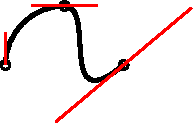
\includegraphics{figures/spline}
  \end{center}
  Hur vill man ange koordinaterna?
  \note[item]{Inget att säga här.}
\end{frame}
\begin{frame}\frametitle{Syntax}
  \begin{itemize}
    \item En kurva byggs upp av sammankopplade \emph{kurvpunkter} \inEnglish{path points} (och delkurvor).\\
      \texttt{pp1{\color{red}-{}-}pp2{\color{red}-{}-}pp3}
    \item En kurvpunkt har en mittpunkt som den interpolerande kurvan passerar genom, och två kontroll-punkter (en framåt och en bakåt).\\
      \texttt{rear{\color{red}<}mid{\color{red}>}front}
    \item Koordinaterna \emph{kan} anges absolut:\\
      \texttt{(0mm,0mm)>(2mm,5mm)\\-{}-(4cm,$\sim$5mm)<(6mm,0mm)>(9mm,3mm)\\-{}-(10mm,0mm)}\\
      \begin{center}
        
\includegraphics{figures/absolute}        
      \end{center}
  \end{itemize}
\end{frame}
\begin{frame}\frametitle{Relativa och polära koordinater}
  \begin{itemize}
  \item Kontroll-punkterna kan anges relativt den mittpunkt de tillhör, och en mittpunkt kan anges relativt föregående mittpunkt på kurvan.
  \item Relativa koordinater kan anges med ett relativ-uttryck:\\
    Båda koordinaterna tillsammans: \texttt{{\color{red}(+}(x,y){\color{red})}}\\
    Var och en för sig: \texttt{(x,{\color{red}(+}y{\color{red})})}
  \item Kontrollpunkter kan även anges relativt på polär form med speciell syntax:\\
    \texttt{{\color{red}(}r{\color{red}\textasciicircum}a{\color{red})}}
  \item I de polära koordinaterna kan endera eller båda komponenterna utelämnas.
  \end{itemize}
\end{frame}
\begin{frame}\frametitle{Semantik}
  Värden för utelämnade komponenter i polära koordinater bestäms i grova drag enligt:
  \begin{itemize}
  \item Vinklar propageras genom mittpunkter (eventuellt hörn).
  \item Resterande vinklar bestäms baserat på mittpunktens läge i förhållande till angränsande mittpunkter.
  \item Radier propageras genom mittpunkter.
  \item Resterande radier beräknas baserat på vinklar.
  \end{itemize}

  Alla effekter är lokala, vilket gör processen lättare att hantera.
\end{frame}
\begin{frame}\frametitle{Smarta enheter}
  När en radie beräknas baserat på vinklar används en \emph{special-enhet} för längd.
  \begin{itemize}
  \item Avbildar mitt-mitt-avstånd och vinklar på radie.
  \item $9$ special-enheter är definierade, och gör det enkelt att approximera cirkelbågar, undvika inflexioner, göra vågor, med mera.
  \item Vilken enhet som används bestäms av \texttt{@specialunit}, men det går också bra att använda special-enheter direkt som radie-angivelse.
  \item Se \filename{pathconstruction.drool}!
  \end{itemize}
\end{frame}
\subsection{Travare}
\frame{\frametitle{Travare}
  En \emph{travare} \inEnglish{slider} är ett kurva--kurvtid-par.
  \begin{itemize}
  \item Skapa utifrån kurvlängd, kurvtid, eller andra beräkningar:\\
    \texttt{[pth 1.3]}, \texttt{[pth 7mm]}, \texttt{pth.begin + 12mm}, \texttt{[continuous\_approximator pth (4cm,7cm)]}
  \item Punktvisa egenskaper för kurvan (i 3D även binormaler):\\
    \texttt{sl.p}, \texttt{sl.v}, \texttt{sl.rv}, \texttt{sl.t}, \texttt{sl.rt}, \texttt{sl.n}, \texttt{sl.rn}, 
    \texttt{sl.ik}, \texttt{sl.rik}, \texttt{sl.time}, \texttt{sl.length}, \texttt{sl.past}, \texttt{sl.looped}, \texttt{sl.mod}
  \item Del-kurvor:\\
    \texttt{[pth 2cm]-{}-[pth 2.5cm]}
  \end{itemize}
  \note[item]{Känns som ett lyckat koncept.}
}
\subsection{Grundläggande grafik}
\begin{frame}\frametitle{Grundläggande kurv-målning}
  För att komma igång med ritandet:
  \begin{itemize}
  \item För att måla kurvor:\\
    \texttt{[{\color{red}stroke} pth]}, \texttt{[{\color{red}fill} pth]}, \texttt{[{\color{red}fillodd} pth]}
  \item Välja färg och dylikt:\\
    \texttt{@stroking}, \texttt{@nonstroking}, \texttt{@width}, \texttt{@dash}, \texttt{@cap}, \texttt{@join}, \texttt{@miterlimit}, \texttt{@blend}, \texttt{@nonstrokingalpha}, \texttt{@strokingalpha}
  \item Utmatning:\\
    \texttt{$\bullet$page <{}< pic1 <{}< pic2 <{}< pic3}
  \end{itemize}
  \note[item]{Inget att säga här.}  
\end{frame}
\begin{frame}\frametitle{Transformationer}
  Transformationer är affina avbildningar som applicerar på grafik och andra geometriska objekt.
  \begin{itemize}
  \item Används som vilken funktion som helst:\\
    \texttt{[tf obj]}
  \item Kan sättas ihop med multiplikationsoperatorn:\\
    \texttt{[tf2*tf1 obj]} = \texttt{[tf2 [tf1 obj]]}
  \item Generella konstruktorer:\\
    \texttt{[affinetransform (1,2) (3,4) (5mm,6mm)]}, \\
    \texttt{[affinetransform3D (1,2,3) (3,4,5) (5,6,7) (8mm,9mm,0mm)]}
  \item Specialiserade konstruktorer:\\
    \texttt{[rotate 25°]}, \texttt{[shift (5mm,0mm)]}, \\
    \texttt{[rotate3D dir:($\sim$1,0,0) angle:45°]}, \texttt{[inverse tf]}\\
    \texttt{[scale 2.5]}, \texttt{[scale y:$\sim$1]}, \texttt{[scale3D x:2 z:3]}
  \end{itemize}
\end{frame}
\begin{frame}\frametitle{Grundläggande text-målning}
  \Shapes har stöd för de typsnitt som ingår i PDF-standarden.
  \begin{itemize}
  \item Manuell och automatisk kernering(?) \inEnglish{kerning}.
  \item Tyvärr begränsat urval av tecken som kan kodas.  Dock inte sämre än att svenska tecken klarat sig.
  \item Typsnittsegenskaper sätts som vanligt med dynamiska variabler, fångas i regel upp vid kernering.
  \item Grafiken skapas genom att text-operationer samlas i ett tillstånd:\\
    \texttt{( {\color{red}newText} <{}< op1 <{}< op2 )}
  \item En text-operation är oftast en sträng eller en sträng med kernering:\\
    \texttt{( {\color{red}newText} <{}< [kern \textasciigrave{}LINK\textasciiacute{} 0.15 \textasciigrave{}ÖPING\textasciiacute{}] )}\\
    \begin{center}
      
\includegraphics{figures/linkoping}
    \end{center}
  \end{itemize}
\end{frame}
\begin{frame}
  \begin{center}
    \includegraphics[width=0.9\paperwidth]{figures/fontmeterdemo}
  \end{center}
\end{frame}
\subsection{2D}
\begin{frame}\frametitle{Pilhuvuden}
  \begin{itemize}
  \item Pilhuvuden kan sättas i båda ändar av en kurva som ska målas:\\
    \texttt{[stroke pth head:hfn tail:tfn]}
  \item Utseendet definieras av en funktion som avbildar kurvan på ett pilhuvud och ett avstånd som ska klippas bort från kurvan.
  \item I \filename{arrowheads.drext} hittar man bland annat \texttt{metaPostArrow}.
  \item Ett pilhuvud med många parametrar specialiseras typiskt innan det används:\\
    \texttt{myHead: [metaPostArrow ahAngle:60° ...]}
  \end{itemize}
\end{frame}
\begin{frame}\frametitle{Geometriska beräkningar}
  \begin{itemize}
  \item Maximering längs kurva.
  \item Kortaste avstånd kurva--punkt.
  \item Skärning med kurva.
  \end{itemize}
  \note{Inget att säga här.}  
\end{frame}
\begin{frame}
  \begin{center}
    \includegraphics[height=0.9\paperheight]{figures/intersections}
  \end{center}
  \note{Inget att säga här.}  
\end{frame}
\begin{frame}\frametitle{Uppsampling och avbildning}
  Om en kurva ska avildas icke-affint, måste resultatet i regel approximeras.
  \begin{itemize}
  \item Kärnan i \Shapes tillhandahåller inga approximationsmetoder.
  \item Istället uppsampling.
  \item Se \filename{pathmapping.drext}!
  \end{itemize}
  \begin{center}
    \includegraphics[width=0.4\paperheight,angle=90]{figures//sidepaths}
  \end{center}
  \note{Inget att säga här.}  
\end{frame}
\begin{frame}\frametitle{Mer om sampling}
  \begin{itemize}
  \item Uppsampling kan vara ett lätt sätt att krympa onödigt stora bounding boxes.
  \item Nersampling är svårt och finns inte i dagsläget.
  \end{itemize}
\end{frame}
\begin{frame}\frametitle{Genomskinlighet}
  Att hantera genomskinlighet är inte helt okomplicerat.
  \begin{center}
    \includegraphics[height=0.6\paperheight]{figures//blendarrows}
  \end{center}
\end{frame}
\subsection{3D}
\begin{frame}\frametitle{Grundläggande användning}
  \begin{itemize}
  \item Grafik i 3D måste \emph{betraktas} \inEnglish{view} från ett öga i $(0,0,\texttt{@eyez})$ med blicken mot origo, innan den kan kombineras med 2D-världen.
  \item Grafik i 2D kan bäddas in \inEnglish{immerse} i 3D genom att lägga till en $z$-koordinat med värdet noll.
  \item Kurvor i 3D (formen, men inte linjebredden) approximeras till önskad precision när de betraktas.
  \item Streckning \inEnglish{dash} hanteras streck för streck.
  \item (Uppsampling saknas i dagsläget.)
  \end{itemize}
  \note{Inget att säga här.}
\end{frame}
\begin{frame}\frametitle{Geometriska beräkningar}
  \begin{itemize}
  \item Maximering längs kurva.
  \item Kortaste avstånd kurva--punkt.
  \end{itemize}
  \begin{center}
    \includegraphics[height=0.5\paperheight]{figures//approximators3d}
  \end{center}
\end{frame}
\begin{frame}\frametitle{Avancerad användning}
  \begin{itemize}
  \item En yta som färgas av ljusmodellen skapas med \texttt{facet}, och kan förfinas med \texttt{facetnormal}.
  \item Ytor kan vara enkel- (kan spara beräkningar) eller dubbelsidiga (om man är lat).
  \item En \emph{tiebreaker} kan användas för att ordna ytor som ligger i varandra.
  \item Ytor kan ges reflexionsegenskaper:\\
    \texttt{@reflexions}, \texttt{@autointensity}, \texttt{@autoscattering}
  \item Ljuskällor av olika typer:\\
    \texttt{ambient\_light}, \texttt{specular\_light}, \texttt{distant\_light}
  \item Dynamiska parametrar styr upplösning och teknik:\\
    \texttt{@facetresolution}, \texttt{@shadeorder}
  \item Överlap hanteras med två metoder, $z$-buffer och $z$-sortering.
  \end{itemize}
\end{frame}
\begin{frame}
  \begin{center}
    \includegraphics[width=\textwidth]{figures//zbufdemo}
  \end{center}
\end{frame}
{
\setbeamercolor{normal text}{bg=black} 
\begin{frame}
  \begin{center}
    \includegraphics[height=0.8\paperheight]{figures//lightdemo}
  \end{center}
\end{frame}
}
\subsection{PDF}
\begin{frame}\frametitle{PDF}
  \Shapes har stöd för
  \begin{itemize}
  \item Dokument med många sidor.  Varje sida läggs till \texttt{$\bullet$catalog}.
  \item Korsreferenser och dokumentöversikt.
  \item Sidnummer.
  \item Text-tillägg \inEnglish{text annotations}.
  \item Se \filename{multipage.pdf}!
  \end{itemize}
  \note{Inget att säga här.}  
\end{frame}
\subsection{Diverse}
\begin{frame}\frametitle{\LaTeX{} och strängar}
  \begin{itemize}
  \item För att använda pdf\LaTeX{}:\\
%    \texttt{(TeX \textasciigrave{}\$\alpha\$ \% this is a comment\textasciiacute)}
  \item Syntaxen för strängar är noga utformad för att inte hamna i konflikt med \TeX{}.
  \item Ovanliga escape-tecken: \texttt{\cent} och \texttt{\currency}
  \item Undviker onödigt många anrop till pdf\LaTeX{} genom att spara resultat mellan körningar.
  \item Se \filename{boxedeq.drool}!
  \end{itemize}
\end{frame}
\begin{frame}\frametitle{Slumptal}
  Slumptal i ett funktionellt språk?
  \begin{itemize}
  \item Två globala tillstånd utgör inkörsport: \texttt{$\bullet$time} och \texttt{$\bullet$randomdevice}
  \item Funktionerna \texttt{newRandom} och \texttt{devRandom} skapar \emph{slump-frön}.
  \item Ett slump-frö knoppar alltid av sig ett lika dant \emph{slump-tillstånd}, och används normalt sett bara en gång:\\
    \texttt{%
      $\bullet$rand1: [newRandom ($\bullet$time)]\\
      $\bullet$rand2: [devRandom $\bullet$randomdevice]
    }
  \item Slump-tillståndet måste skickas med när man vill ha slumptal:\\
    \texttt{%
      [random2D $\bullet$rand1]
    }
  \item Funktionellt, om än inte jätte-smidigt!
  \end{itemize}
\end{frame}

\section{Utmaningar för framtiden}
\frame{%
  \begin{center}
    {\Huge Utmaningar för framtiden}
  \end{center}
  \note[item]{Inget att säga här.}
}

\frame{\frametitle{Trixelering}
  Att rendera 3D genom en $z$-buffer kompliceras enormt av att det inte finns ett givet raster.
  \begin{itemize}
  \item Analysera vilka och hur många toleranser som måste sättas.
  \item Designa algoritm utifrån invarianter.
  \item Implementera\ldots
  \item Kan även användas för skuggor!
  \end{itemize}
}
\frame{\frametitle{Kompilera funktioner till PDF}
  Just nu används färgövergångar endast vid en viss typ av ljussättning.
  \begin{itemize}
  \item Användaren vill kunna göra egna övergångar.
  \item Funktioner från åskådliga planet till färgrummet ska kunna definieras på hög nivå.
  \item Funktionerna ska fungera som vanligt i \Shapes, men också gå att kompilera till PDF!
  \item Mycket begränsad PostScript-kalkylator.
  \end{itemize}
}
\frame{\frametitle{Bättre stöd för typsnitt}
  Snart lessnar man på de inbyggda typsnitten och begränsningar i teckenkodning.
  \begin{itemize}
  \item Reda ut hur man hanterar teckenkodningen systematiskt.
  \item Förmodligen ta hjälp av FreeType.
  \end{itemize}
}
\frame{\frametitle{Mer grund-struktur}
  \begin{itemize}
  \item Namespaces/packages.
  \item Användar-typer (och -tillstånd!).
  \end{itemize}
  \note[item]{Inget att säga här.}
}

\section{Sammanfattning}
\frame{%
  \begin{center}
    {\Huge Sammanfattning}
  \end{center}
  \note[item]{Inget att säga här.}
}
\frame{\frametitle{Sammanfattning}
  Seminariet har förhoppningsvis förmedlat något om\ldots
  \begin{itemize}
    \item \Shapes ursprung och sammanhang idag.
    \item Språkets grundelement.
    \item Funktionalitet i kärnan.
    \item Hur \Shapes-kod kan se ut.
    \item Hur kompilatorn används.
  \end{itemize}
  \note[item]{Inget att säga här.}
}

\frame{%
  \begin{center}
    \includegraphics[height=0.8\paperheight]{figures//kjmrobot}
  \end{center}
  \note[item]{Tacka för uppmärksamheten!}
}

\end{document}
